\documentclass[12pt]{article}
\usepackage{fullpage}
\usepackage[margin=1in]{geometry}
\usepackage[stable]{footmisc}
\usepackage{graphicx}
\usepackage{amssymb}
\usepackage{IEEEtrantools}
\usepackage{lineno}
\usepackage{amsmath}
\usepackage{epstopdf}
\usepackage{parskip}
\usepackage{authblk}
\usepackage[authoryear]{natbib}
%\setlength{\parskip}{20pt}
\linespread{1.6}
\date{}

\DeclareGraphicsRule{.tif}{png}{.png}{`convert #1 `dirname #1`/`basename #1 .tif`.png}


%%	math short-cuts
\def \ve{\varepsilon}	% epsilon used for metabolic rate
\def \la{\lambda}	% lambda
\newcommand{\eref}[1]{(\ref{#1})}

%%	new commands for referencing figures and tables and sections
\newcommand{\fref}[1]{Figure~\ref{#1}}	% inline figure ref
\newcommand{\fpref}[1]{Fig.~\ref{#1}}	% parenthetical figure ref
\newcommand{\tref}[1]{Table~\ref{#1}}	% table ref
\newcommand{\sref}[1]{Section~\ref{#1}}	% table ref
%\linenumbers

\title{\Large \textbf{Predator prey interaction with MERA III}}

\author{Jade, Oct 31}

\begin{document}
\maketitle
\raggedright
\large
\setlength{\parindent}{15pt}

\section{Growth functions for one predator feeding on one prey}

With the MERA III framework (write-up Oct 13) I have proved that the growth function for one species without competitors or predators is 
  \begin{equation}
 \begin{split}
g =  \frac{r (1 - \frac{N}{\hat {N}})}{1 + (r-1) \frac{N}{\hat {N}}} \hskip 1cm \mbox{(partial redistribution)}\\
= \frac{ r(1- \frac{N }{\hat{N}})} {1+ r \frac{N }{\hat{N}}}\hskip 1cm \mbox{(complete redistribution)}
\end{split}
\end{equation}

For the predator, it has to be a complete redistribution scenario (please refer to Oct 13 write up for definitions; as opposed to the complete redistribution scenario, partial redistribution does not allow abundance to decrease since all resources obtained by the existing population cannot be lost). In this scenario, $\hat {N} = \frac{r R_0 }{(r+1) \theta}$, therefore
  \begin{equation}
 \begin{split}
g =  \frac{r R_0 - (r+1) \theta N}{R_0 + (r+1) \theta N} 
\end{split}
\end{equation}

By convention of predator prey models, in all following equations, $X$ represents the abundance of the the prey while $Y$ represents the abundance of the predator; subscript $x$ indicates prey variables while subscript $y$ indicates predator variables. 

First I will derive the growth function for the predator species. $R_{0,y}$ is the total amount of prey biomass available for the predator,
  \begin{equation}
 \begin{split}
R_{0,y}  = \theta_{x}X
\end{split}
\end{equation}

Substituting into Eq. 2, the per capita net growth rate of the predator $g_y$ can be expressed as:
  \begin{equation}
 \begin{split}
g_y =  \frac{r_y \theta_{x}X  - (r_y+1) \theta_y Y}{\theta_{x}X + (r_y+1) \theta_y Y} 
\end{split}
\end{equation}

For the prey, here we assume that the prey also follows a complete redistribution scenario (but not necessarily, see Appendix for the partial scenario). Before predation happens, the per capita net growth rate of the prey $g_{x,before}$ is 

  \begin{equation}
 \begin{split}
g_{x, before} =  \frac{r_x R_0 - (r_x+1) \theta_x X}{R_0 + (r_x+1) \theta_x X} 
\end{split}
\end{equation}

The prey biomass consumed by the predator $R_{consumed}$ is 
 \begin{equation}
 \begin{split}
R_{consumed}  = \theta_y Y
\end{split}
\end{equation}
Therefore the growth function of the prey after predation should take this into account
 \begin{equation}
 \begin{split}
\theta_x X (g_{x} +1) =\theta_x X (g_{x, before} +1) - R_{consumed}  \\
=> g_{x} = g_{x, before} - \frac{R_{consumed}}{\theta_x X} \\
= \frac{r_x R_0 - (r_x+1) \theta_x X}{R_0 + (r_x+1) \theta_x X} - \frac{\theta_y Y}{\theta_x X}
\end{split}
\end{equation}

Eqs 4 and 7 can be simplified into
 \begin{equation}
 \begin{split}
g_y = \frac{r_{y}  [ 1 -  \theta  \frac{(r_{y} +1)Y}{r_y X} ]}{ 1+ (r_{y}+1) \theta \frac{Y}{X}} 
\end{split}
\end{equation}
 \begin{equation}
 \begin{split}
g_x = \frac{r_{x}  [1 -\frac{(r_{x} +1)X\theta_x}{r_x R_0 }]}{ 1 +  \frac{(r_{x} +1)X\theta_x}{R_0}}   -  \theta\frac{Y}{X} 
\end{split}
\end{equation}

Where $\theta = \theta_P/\theta_p$. Since by definition $g_y = \frac{d Y}{Y d t} $ and $g_x = \frac{d X}{X d t} $, they each correspond to:

 \begin{equation}
 \begin{split}
\frac{d Y}{d t} =g_y \times Y = \frac{r_{y} Y [ 1 -  \theta  \frac{(r_{y} +1)Y}{r_y X} ]}{ 1+ (r_{y}+1) \theta \frac{Y}{X}} 
\end{split}
\end{equation}
 \begin{equation}
 \begin{split}
 \frac{d X}{d t}= g_x \times X =\frac{r_{x} X [1 -\frac{(r_{x} +1)X\theta_x}{r_x R_0 }]}{ 1 +  \frac{(r_{x} +1)X\theta_x}{R_0}}   -  \theta Y
\end{split}
\end{equation}
With Eqs. 10 - 11, population dynamics for both the prey and the predator can be modeled. The following graph shows how the pattern varies when the magnitude of the intrinsic growth rates $r_x$ and $r_y$ increases.

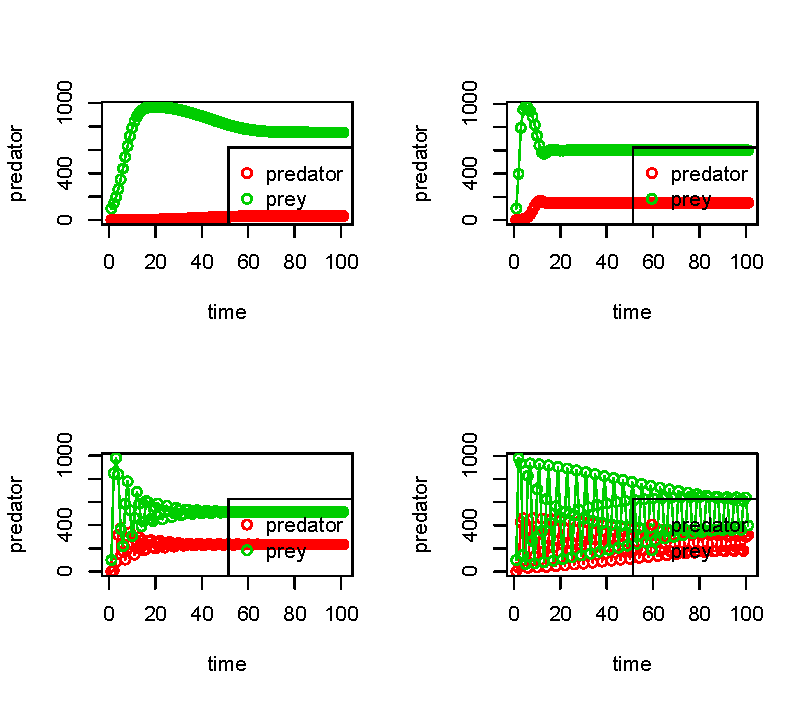
\includegraphics[width=\textwidth]{predator-prey-dynamics.pdf}

($\theta =2, X_0=100, Y_0 = 1$, top left: $r_1=0.1,r_2 = 0.5$, topright: $r_1=1,r_2 = 5$, bottomleft: $r_1=10,r_2 = 50$, bottomright: $r_1=100,r_2 = 500$; environment carrying capacity for the prey $\frac{r_x R_0}{(r_x+1)\theta_x}$ controlled to be 1000.)

\section{Future directions: what to do from here}
\subsection{Building on the current model}
First, I can add more trophic levels and try to reveal the dynamics of multiple species along a food chain. This might be a must if the data contains multiple ($>2$) trophic levels.

Second, I can also reveal the dynamics for multiple competitors at one trophic level (with or without predator). Potentially this will yield equations that resemble the generalized Lotka-Volterra equations under certain circumstances (possibly depending on $D_r$). However, this is less testable due to the open definition and lack of measurement for $D_r$. Before we can more precisely pin $D_r$ down, the best we can do is make general inferences like compare when $D_r=0$ vs when $D_r=1$.

\subsection{Data test}

The Lotka-Volterra predator-prey equations are

 \begin{equation}
 \begin{split}
\frac{d Y}{d t} =\alpha X - \beta XY
\end{split}
\end{equation}
 \begin{equation}
 \begin{split}
 \frac{d X}{d t}= \sigma XY - \gamma Y 
\end{split}
\end{equation}

Eqs. 10 - 11 have the same amount of parameters as The Lotka-Volterra predator-prey equations ($r_x$, $r_y$, $\theta$, $R_0$). However, the physical meanings of MERA parameters are much clearer: $r_x$ and $r_y$ are each the intrinsic growth rates for the prey or the predator when food is unlimited, $\theta$ is the ratio between their metabolic rates, $R_0$ is amount of total fundamental resource for the prey. They can be measured and compared between systems with different species composition (e.g. a prey-only system vs a predator-prey system). This way the MERA solutions can be explicitly tested. In summary, it will be ideal if we can find dataset(s) that satisfy the following requirements:

1. Time series of predator and prey population sizes;

2. Body sizes or metabolic rates of both species can be estimated;

3. For the same environment, prey dynamics when there is no predator (to acquire $r_x$ and $R_0$);

4. For the same environment, predator dynamics when prey is abundant (to acquire $r_y$ and $\theta$).

With only 1, it is probably hard to distinguish MERA solutions from the Lotka-Volterra equations. But with 2-4 in addition, it will be a much stronger test. Given the above, I think the microcosm experiments are my best bet. Please advise me if you have information and/or thoughts on this.

\section{Appendix: When the prey follows a partial redistribution scenario}
The per capita net growth rate of the prey will be different:
 \begin{equation}
 \begin{split}
g_x = \frac{r_{x}  (1 -\frac{X\theta_x}{R_0 })}{ 1 +  \frac{(r_{x}-1)X\theta_x}{R_0}}   -  \theta\frac{Y}{X} 
\end{split}
\end{equation}

 \begin{equation}
 \begin{split}
 \frac{d X}{d t}= g_x \times X = \frac{r_{x} X  (1 -\frac{X\theta_x}{R_0 })}{ 1 +  \frac{(r_{x}-1)X\theta_x}{R_0}}   -  \theta Y
\end{split}
\end{equation}

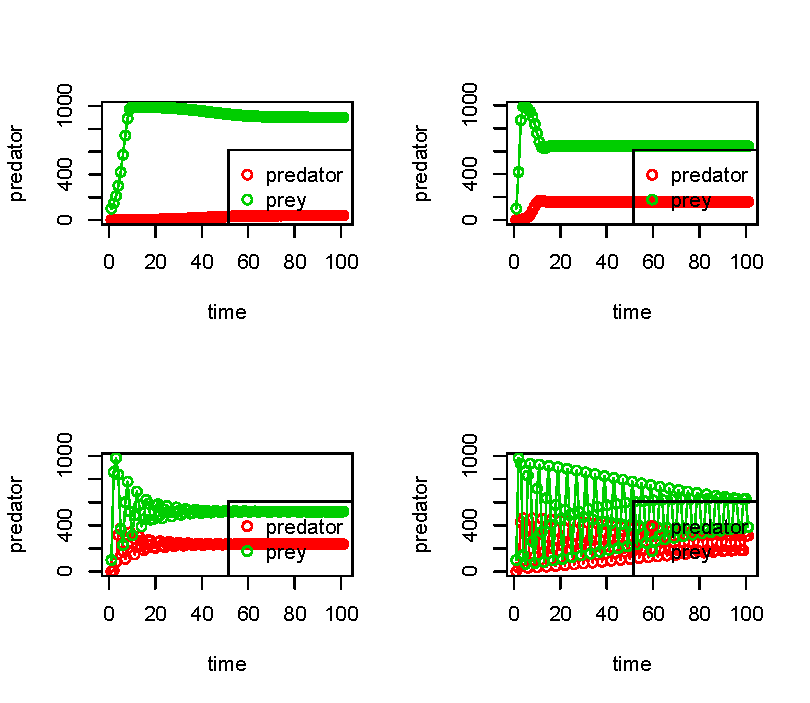
\includegraphics[width=\textwidth]{predator-prey-dynamics-partial.pdf}

Same parameter setting as the first graph.

\end{document}